%! Author = Len Washington III
%! Date = 11/05/2023

% Preamble
\documentclass[24]{cs430lecture}

% Packages

% Document
\begin{document}

%<*Lecture-Activity-24>
\let\oldsout\sout
\renewcommand{\sout}[1]{\textcolor{red}{#1}}
\newcommand{\queuesep}{\ \ \ }
\newcommand{\queuepathset}[1][.]{
	\ifinanswer%
	\colorlet{current}{blue}%
	\else%
	\colorlet{current}{#1}%
	\fi%
	\tikzset{>={Stealth[current]},
		every node/.style={current,fill=white,circle},
		every edge/.style={current,thin,draw},
		used/.style={orange,very thick,draw}}%draw=current instead of current,draw?
}
\newcommand{\queuenodeset}[1][.]{
	\ifinanswer%
	\colorlet{current}{blue}%
	\else%
	\colorlet{current}{#1}%
	\fi%
	\tikzset{every node/.style={circle,thick,draw},
	every gray/.style={fill=white!80!black},
	every black/.style={fill=white!40!black},
	}%draw=current instead of current,draw?
}
\maketitle
\begin{answer}
	Relationships between items:
	\begin{description}
		\item[$\mathbf{1-1}$] List, Stack, Queue
		\item[$\mathbf{1-N}$] Tree, Hierarchical
		\item[$\mathbf{N-N}$] Any graph item can be related to any other item.
	\end{description}
\end{answer}
\openingquestions

\begin{enumerate}
    \item Give an example NOT discussed in the video lecture of a problem that can be represented by a graph.
	\begin{answer}The connections between airports.\end{answer}
	\item If there is a path in a graph from a vertex back to itself, that is called a
	\begin{answer}\underline{cycle}%
	\footnote{A path of one edge is called a self-loop.}\end{answer}.
	\item Which representation of a graph, adjacency-list and adjacency-matrix, usually uses more memory and why?
	\begin{answer}The adjacency-matrix usually uses more memory than the adjacency-list because the adjacency matrix represents both the existence of edges and the non-existence of edges.\end{answer}
\end{enumerate}

\section{Graphs}\label{sec:graphs}
\begin{enumerate}
    \item Draw the graph:
	A directed graph $G=(V,E)$ where $V=\{ 1, 2, 3, 4, 5, 6 \}$ and $E=\{ (1,2), (2,2), (2,4), (2,5), (4,1), (4,5), (5,4), (6,3) \}$.
	What is the edge $(2,2)$ called?
	\begin{answer}
		\begin{figure}[H]
			\centering
			\begin{tikzpicture}
				\begin{scope}\globalnodeset
					\node (1) at (0,0) {1};
					\node (2) at (3,0) {2};
					\node (3) at (6,0) {3};
					\node (4) at (0,-3) {4};
					\node (5) at (3,-3) {5};
					\node (6) at (6,-3) {6};
				\end{scope}
				\begin{scope}\globalpathset
					\path [->] (1) edge (2);

					\path [->] (2) edge[loop above] (2);
					\path [->] (2) edge (4);
					\path [->] (2) edge (5);

					\path [->] (4) edge (1);
					\path [->] (4) edge[bend left=10] (5);

					\path [->] (5) edge[bend left=10] (4);

					\path [->] (6) edge (3);
				\end{scope}
			\end{tikzpicture}
			\label{fig:24-draw-1}
		\end{figure}
		The edge $(2,2)$ is a self-loop.
	\end{answer}
	\item Draw the graph:
	An undirected graph $G=(V,E)$ where $V=\{ 1, 2, 3, 4, 5, 6 \}$ and $E=\left\{ \{1,2\}, \{ 1, 5\}, \{ 2, 5\}, \{ 3, 6\} \right\}$.
	What is vertex $4$ called?
	What is the difference about how an edge set $E$ is denoted for an undirected graph?
	Are self-loops allowed in an undirected graph?
	\begin{answer}
		\begin{figure}[H]
			\centering
			\begin{tikzpicture}
				\begin{scope}\globalnodeset
					\node (1) at (0,0) {1};
					\node (2) at (3,0) {2};
					\node (3) at (6,0) {3};
					\node (4) at (0,-3) {4};
					\node (5) at (3,-3) {5};
					\node (6) at (6,-3) {6};
				\end{scope}
				\begin{scope}\globalpathset
					\path (1) edge (2);
					\path (1) edge (5);

					\path (2) edge (5);

					\path (3) edge (6);
				\end{scope}
			\end{tikzpicture}
			\label{fig:24-draw-2}
		\end{figure}
		A vertex that is has no edges (is not connected to anything) is isolated.%
		\footnote{In a directed graph, if the only connection a node has is to itself (a self-loop), then it is still considered isolated.}
		The difference between how an edge set $E$ is denoted for an undirected graph versus a directed graph is that the directed graph is a tuple (where order matters) while an undirected graph is a set (where order doesn't matter).
		Self-loops are not allowed in an undirected graphs.
	\end{answer}
	\item Define these terms:
	\begin{itemize}
		\item Vertex $v$ is adjacent to vertex $u$ in an undirected graph.
		\begin{answer} There is an edge $\{ u, v\}$ (which is equivalent to $\{ v, u\}$). \end{answer}
		\item Vertex $v$ is adjacent to vertex $u$ in a directed graph.
		\begin{answer} $(u,v): u\rightarrow v$, which is not the same as $(v,u)$. \end{answer}
		\item The degree of a vertex in an undirected graph.
		\begin{answer} The number of edges touching the vertex. \end{answer}
		\item The degree of a vertex in a directed graph.
		\begin{answer} There are two types of degrees.
			\begin{description}
				\item[Out Degree] The number of edges leaving the vertex.
				\item[In Degree] The number of edges entering the vertex.
			\end{description}
			The total degree is the sum of the In Degrees and Out Degrees.
		\end{answer}
		\item A path in an undirected graph.
		\begin{answer} Sequences of edges from a vertex to a vertex where the reuse of edges is okay. \end{answer}
		\item A path in a directed graph.
		\begin{answer} Sequence of edges in order of ordered pairs (following arrows). \end{answer}
		\item The length of a path.
		\begin{answer} The number of edges on the path. \end{answer}
		\item $v$ is reachable from $u$.
		\begin{answer} There is a path from $u$ to $v$. \end{answer}
		\item A simple path.
		\begin{answer} A path with no reused vertices OR edges.\end{answer}
		\item A cycle in an undirected graph.
		What about a simple cycle?
		\begin{answer} The path from a vertex to itself.
		A simple cycle is a cycle that doesn't reuse vertices or edges to get back to the original vertex
		(simple path back to the same vertex).\end{answer}
		\item A cycle in a directed graph.
		What about a simple cycle?
		\begin{answer} The path in the ordered direction from a vertex to itself. \end{answer}
		\item Acyclic graph.
		\begin{answer} No cycles in the graph. \end{answer}
		\item Connected undirected graph.
		\begin{answer} Every vertex is reachable from every other vertex. \end{answer}
		\item Connected directed graph.
		\begin{answer} Also known as a strongly connected graph.
		Every vertex is reachable (along edges in the correct direction) from every other vertex.\end{answer}
		\item Bipartite Graph.
		\begin{answer} Separate the vertices into 2 sets.
		All edges go between the 2 sets.
		There are no edges between vertices in the same set.\end{answer}
	\end{itemize}
\end{enumerate}

\section{Graph Implementations}\label{sec:graph-implementations}
\begin{enumerate}[start=4]
    \item What is the adjacency list implementation of these two graphs?

	\begin{minipage}[t]{0.5\textwidth}
		\begin{figure}[H]
			\centering
			\begin{tikzpicture}
				\begin{scope}\globalnodeset
				\node (1) at (0,0) {1};
				\node (2) at (3,0) {2};
				\node (3) at (5,-1.5) {3};
				\node (4) at (3,-3) {4};
				\node (5) at (0,-3) {5};
				\end{scope}

				\begin{scope}\globalpathset
				\path (1) edge (2);
				\path (1) edge (5);

				\path (2) edge (3);
				\path (2) edge (4);
				\path (2) edge (5);

				\path (3) edge (4);
				\path (4) edge (5);
				\end{scope}
			\end{tikzpicture}
			\label{fig:24.1}
		\end{figure}
		\begin{answer}
			\begin{table}
			    \centering
			    \begin{threeparttable}
					\label{tab:adjacency-list-a}
					\begin{tabular}{|c|l}
					\toprule
					1 & $\rightarrow5\rightarrow2$\\
					\midrule
					2 & $\rightarrow1\rightarrow5\rightarrow4$\\
					\midrule
					3 & $\rightarrow2\rightarrow4$\\
					\midrule
					4 & $\rightarrow2\rightarrow3\rightarrow5$\\
					\midrule
					5 & $\rightarrow1\rightarrow2\rightarrow4$\\
					\bottomrule
				\end{tabular}
					\begin{tablenotes}
						\small
						\item No order to the list of vertices.
						\item The arrows are representing a linked list of who the vertex is connected to (NOT a set of edges.)
					\end{tablenotes}
				\end{threeparttable}
			\end{table}
		\end{answer}
	\end{minipage}\begin{minipage}[t]{0.5\textwidth}
		\begin{figure}[H]
			\centering
			\begin{tikzpicture}
				\begin{scope}\globalnodeset
					\node (1) at (0,0) {1};
					\node (2) at (3,0) {2};
					\node (3) at (6,0) {3};
					\node (5) at (0,-3) {5};
					\node (4) at (3,-3) {4};
					\node (6) at (6,-3) {6};
				\end{scope}
				\begin{scope}\globalpathset
					\path [->] (1) edge (2);
					\path [->] (1) edge (5);

					\path [->] (2) edge (4);

					\path [->] (3) edge (2);
					\path [->] (3) edge (6);

					\path [->] (4) edge (5);
					\path [->] (4) edge[bend left=10] (6);

					\path [->] (6) edge[bend right=350] (4);
				\end{scope}
			\end{tikzpicture}
			\label{fig:24.2}
		\end{figure}
		\begin{answer}
			\begin{table}
			    \centering
				\label{tab:adjacency-list-b}
				\begin{tabular}{|c|l}
					\toprule
					1 & $\rightarrow2\rightarrow5$\\
					\midrule
					2 & $\rightarrow4$\\
					\midrule
					3 & $\rightarrow2\rightarrow6$\\
					\midrule
					4 & $\rightarrow5\rightarrow6$\\
					\midrule
					5 & \\
					\midrule
					6 & $\rightarrow4$\\
					\bottomrule
				\end{tabular}
			\end{table}
		\end{answer}
	\end{minipage}
	\begin{answer}Memory: $O(|V| + |E|)$.
	Find if edge exists: $O(|V|)$.
	Remember, the amount of memory needed for the undirected graph is greater for the undirected graph than the directed graph,
	since each edge in the undirected graph is represented twice, while each edge in the directed graph is represented once.
	Find the path using the adjacency list is $O(|V|^{2})$.\end{answer}
	\item What is the adjacency matrix implementation of the above two graphs?
	\begin{answer}Memory: $O(|V|^{2})$,
	Time to find if a path exists: $O(1)$.
	Can find the path using the adjacency matrix, learn that \hyperref[sec:all-pairs-shortest-paths-problem]{later}.

		\begin{minipage}[t]{0.45\textwidth}
			\begin{table}
				\centering
				\label{tab:adjacency-matrix-1}
				\begin{tabular}{cccccc}
					  & 1 & 2 & 3 & 4 & 5\\
					1 & 0 & 1 & 0 & 0 & 1\\
					2 & 1 & 0 & 1 & 1 & 1\\
					3 & 0 & 1 & 0 & 1 & 0\\
					4 & 0 & 1 & 1 & 0 & 1\\
					5 & 1 & 1 & 0 & 1 & 0
				\end{tabular}
			\end{table}
			The adjacency matrix for an undirected graph should have all 0's on its main diagonal.
			A 1 implies a self-loop which wouldn't be allowed.
		\end{minipage}\begin{minipage}[t]{0.55\textwidth}
			\begin{table}
				\centering
				\label{tab:adjacency-matrix-2}
				\begin{tabular}{ccccccc}
					  & 1 & 2 & 3 & 4 & 5 & 6\\
					1 & 0 & 1 & 0 & 0 & 1 & 0\\
					2 & 0 & 0 & 0 & 1 & 0 & 0\\
					3 & 0 & 1 & 0 & 0 & 0 & 1\\
					4 & 0 & 0 & 0 & 0 & 1 & 1\\
					5 & 0 & 0 & 0 & 0 & 0 & 0\\
					6 & 0 & 0 & 0 & 1 & 0 & 0\\
				\end{tabular}
			\end{table}
		\end{minipage}
	\end{answer}
	\item How do the two implementations handle a weighted graph?
	\begin{answer}Edges have numbers, add weights to the adjacency matrix instead of the boolean values of 1/0 representing if there is a weight.
	If you're using an adjacency list, then each item will have the be an object holding the vertex and the weight to that vertex, instead of just using the vertex label as the element.\end{answer}
	\item Two different representations of the graph data structure are discussed in the book, adjacency-list and adjacency-matrix.
	Please briefly discuss the runtime (in terms of $|V|$ and $|E$ of these graph operations/algorithms using each implementation.)
	Assume vertices are labeled as integers.
	\begin{itemize}
		\item What is the worst-case big-O runtime for checking to see if an edge from vertex $u$ to vertex $v$ exists?
		\begin{answer}Adj list: $O(|V|)$, Adj matrix: $O(1)$\end{answer}
		\item How long does it take to compute the out-degree of every vertex of a directed graph?
		\begin{answer} In the adjacency list, you would keep track of it in the item and add or subtract from it when an edge is added or removed.
		In an adjacency matrix, you would count the number of non-zeroes in each row.\end{answer}
		\item How long does it take to compute the in-degree of every vertex of a directed graph?
		\begin{answer}In an adjacency matrix, you would count the number of non-zeroes in each column.
		In the adjacency matrix, you would have to go through each vertices linked list and check if it connects to 4.\end{answer}
	\end{itemize}
\end{enumerate}

\section{Graph Traversals}\label{sec:graph-traversals}
A way to search/visit all the vertices in a graph.
There is not a unique answer usually.
\begin{itemize}
	\item Undirected graph - if connected, all vertices will be visited.
	\item Directed graph - Must be strongly connected to be able to visit all vertices.
\end{itemize}

Breadth first\label{dfn:breadth-first-search} - visit vertices one edge from a given (or random) source, two edges from source, etc.
Uses a queue and some way to make a vertex (white initially, gray when first visited and put in queue, black when out of queue),
label a vertex how far from the source, and label a vertex with how its predecessor vertex was during the traversal.

\begin{enumerate}[start=8]
    \item Perform a breadth first search on this graph.
	\begin{figure}[H]
		\centering
		\graphexample
		\label{fig:24.3}
	\end{figure}
	\begin{answer}
		\begin{itemize}
			\item Random source
			\item Every vertex unvisited (white)
			\item When first visit a vertex
			\begin{itemize}
				\item Add to queue
				\item Color it gray
			\end{itemize}
			\item When done with vertex
			\begin{itemize}
				\item Color vertex black
				\item Remove from queue
			\end{itemize}
		\end{itemize}
		Warning: Bauer forgot about the $(E,A)$ connection in the example he did, so while I drew it, it was not brought into consideration.

		\begin{minipage}{0.5\textwidth}
			\begin{figure}[H]
				\centering
				\begin{tikzpicture}
					\begin{scope}\queuenodeset
						\node (A) at (0,0) {$A$};
						\node (B) at (2,-2) {$B$};
						\node (C) at (3.5,2) {$C$};
						\node[label=45:``Random Source'':$D$,black] (D) at (6,0.5) {$D$};
						\node (E) at (6,-2.5) {$E$};
						\node (F)[gray] at (8,-0.25) {$F$};
					\end{scope}
					\begin{scope}\queuepathset
						\path [->] (A) edge (C);

						\path [->] (B) edge (A);
						\path [->] (B) edge[bend right=7] (C);
						\path [->] (B) edge (D);

						\path [->] (C) edge[bend right=7] (B);
						\path [->] (C) edge (D);

						\path [->] (D) edge[used] (F);

						\path [->] (E) edge (B);
						\path [->] (E) edge[bend left=80] (A);

						\path [->] (F) edge (E);
					\end{scope}
				\end{tikzpicture}
				\caption{Queue: $F^{1} \queuesep \sout{D^{0}}$}
				\label{fig:queue-1}
			\end{figure}
		\end{minipage}\begin{minipage}{0.5\textwidth}
			\begin{figure}[H]
				\centering
				\begin{tikzpicture}
					\begin{scope}\queuenodeset
						\node (A) at (0,0) {$A$};
						\node (B) at (2,-2) {$B$};
						\node (C) at (3.5,2) {$C$};
						\node[label=45:``Random Source'':$D$,black] (D) at (6,0.5) {$D$};
						\node (E)[gray] at (6,-2.5) {$E$};
						\node (F)[black] at (8,-0.25) {$F$};
					\end{scope}
					\begin{scope}\queuepathset
						\path [->] (A) edge (C);

						\path [->] (B) edge (A);
						\path [->] (B) edge[bend right=7] (C);
						\path [->] (B) edge (D);

						\path [->] (C) edge[bend right=7] (B);
						\path [->] (C) edge (D);

						\path [->] (D) edge[used] (F);

						\path [->] (E) edge (B);
						\path [->] (E) edge[bend left=80] (A);

						\path [->] (F) edge[used] (E);
					\end{scope}
				\end{tikzpicture}
				\caption{Queue: $E^{2} \queuesep \sout{F^{1}} \queuesep \sout{D^{0}}$}
				\label{fig:queue-2}
			\end{figure}
		\end{minipage}
		\begin{minipage}{0.5\textwidth}
			\begin{figure}[H]
				\centering
				\begin{tikzpicture}
					\begin{scope}\queuenodeset
						\node (A) at (0,0) {$A$};
						\node[gray] (B) at (2,-2) {$B$};
						\node (C) at (3.5,2) {$C$};
						\node[label=45:``Random Source'':$D$,black] (D) at (6,0.5) {$D$};
						\node[black] (E) at (6,-2.5) {$E$};
						\node[black] (F) at (8,-0.25) {$F$};
					\end{scope}
					\begin{scope}\queuepathset
						\path [->] (A) edge (C);

						\path [->] (B) edge (A);
						\path [->] (B) edge[bend right=7] (C);
						\path [->] (B) edge (D);

						\path [->] (C) edge[bend right=7] (B);
						\path [->] (C) edge (D);

						\path [->] (D) edge[used] (F);

						\path [->] (E) edge[used] (B);
						\path [->] (E) edge[bend left=80] (A); % FIXME: Just realized Bauer excluded the E->A edge

						\path [->] (F) edge[used] (E);
					\end{scope}
				\end{tikzpicture}
				\caption{Queue: $B^{3} \queuesep \sout{E^{2}} \queuesep \sout{F^{1}} \queuesep \sout{D^{0}}$}
				\label{fig:queue-3}
			\end{figure}
		\end{minipage}\begin{minipage}{0.5\textwidth}
			\begin{figure}[H]
				\centering
				\begin{tikzpicture}
					\begin{scope}\queuenodeset
						\node[gray] (A) at (0,0) {$A$};
						\node[black] (B) at (2,-2) {$B$};
						\node[gray] (C) at (3.5,2) {$C$};
						\node[label=45:``Random Source'':$D$,black] (D) at (6,0.5) {$D$};
						\node[black] (E) at (6,-2.5) {$E$};
						\node[black] (F) at (8,-0.25) {$F$};
					\end{scope}
					\begin{scope}\queuepathset
						\path [->] (A) edge (C);

						\path [->] (B) edge[used] (A);
						\path [->] (B) edge[bend right=7,used] (C);
						\path [->] (B) edge (D);

						\path [->] (C) edge[bend right=7] (B);
						\path [->] (C) edge (D);

						\path [->] (D) edge[used] (F);

						\path [->] (E) edge[used] (B);
						\path [->] (E) edge[bend left=80] (A);

						\path [->] (F) edge[used] (E);
					\end{scope}
				\end{tikzpicture}
				\caption{Queue: $C^{4} \queuesep A^{4} \queuesep \sout{B^{3}} \queuesep \sout{E^{2}} \queuesep \sout{F^{1}} \queuesep \sout{D^{0}}$}
				\label{fig:queue-4}
			\end{figure}
		\end{minipage}
		\begin{minipage}{0.5\textwidth}
			\begin{figure}[H]
				\centering
				\begin{tikzpicture}
					\begin{scope}\queuenodeset
						\node[black] (A) at (0,0) {$A$};
						\node[black] (B) at (2,-2) {$B$};
						\node[gray] (C) at (3.5,2) {$C$};
						\node[label=45:``Random Source'':$D$,black] (D) at (6,0.5) {$D$};
						\node[black] (E) at (6,-2.5) {$E$};
						\node[black] (F) at (8,-0.25) {$F$};
					\end{scope}
					\begin{scope}\queuepathset
						\path [->] (A) edge (C);

						\path [->] (B) edge[used] (A);
						\path [->] (B) edge[bend right=7,used] (C);
						\path [->] (B) edge (D);

						\path [->] (C) edge[bend right=7] (B);
						\path [->] (C) edge (D);

						\path [->] (D) edge[used] (F);

						\path [->] (E) edge[used] (B);
						\path [->] (E) edge[bend left=80] (A);

						\path [->] (F) edge[used] (E);
					\end{scope}
				\end{tikzpicture}
				\caption{Queue: $C^{4} \queuesep \sout{A^{4}} \queuesep \sout{B^{3}} \queuesep \sout{E^{2}} \queuesep \sout{F^{1}} \queuesep \sout{D^{0}}$}
				\label{fig:queue-5}
			\end{figure}
		\end{minipage}\begin{minipage}{0.5\textwidth}
			\begin{figure}[H]
				\centering
				\begin{tikzpicture}
					\begin{scope}\queuenodeset
						\begin{scope}\queuenodeset
						\node[black] (A) at (0,0) {$A$};
						\node[black] (B) at (2,-2) {$B$};
						\node[black] (C) at (3.5,2) {$C$};
						\node[label=45:``Random Source'':$D$,black] (D) at (6,0.5) {$D$};
						\node[black] (E) at (6,-2.5) {$E$};
						\node[black] (F) at (8,-0.25) {$F$};
					\end{scope}
					\end{scope}
					\begin{scope}\queuepathset
						\path [->] (A) edge (C);

						\path [->] (B) edge[used] (A);
						\path [->] (B) edge[bend right=7,used] (C);
						\path [->] (B) edge (D);

						\path [->] (C) edge[bend right=7] (B);
						\path [->] (C) edge (D);

						\path [->] (D) edge[used] (F);

						\path [->] (E) edge[used] (B);
						\path [->] (E) edge[bend left=80] (A);

						\path [->] (F) edge[used] (E);
					\end{scope}
				\end{tikzpicture}
				\caption{Queue: $\sout{C^{4}} \queuesep \sout{A^{4}} \queuesep \sout{B^{3}} \queuesep \sout{E^{2}} \queuesep \sout{F^{1}} \queuesep \sout{D^{0}}$}
				\label{fig:queue-6}
			\end{figure}
		\end{minipage}
		\begin{figure}[H]
			\centering
			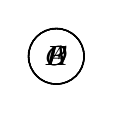
\begin{tikzpicture}
				\tikzset{every node/.style={minimum width=2em,draw,circle},
					 blank/.style={draw=none},
					 edge from parent/.style=
					 {draw,edge from parent path={(\tikzparentnode) -> (\tikzchildnode)}},
					 level distance=1cm,
					sibling distance=5mm}
				\Tree
				[.\node{ $D$ };
					[.\node{ $F$ };
						[.\node{ $E$ };
							[.\node{ $B$ };
								[.\node{ $A$ }; ]
								[.\node{ $C$ }; ]
							]
						]
					]
				]
			\end{tikzpicture}
			\caption{Breadth First Tree from Source $D$. Shows the shortest path (minimum \# edges) from each vertex to the source.}
			\label{fig:bfs-tree}
		\end{figure}
		Breadth-first search gives us the minimum \# of edges to every vertex reachable from the source.
	\end{answer}
\end{enumerate}

\begin{algorithm}[H]
	\caption{Breadth-First Search for Graphs}\label{alg:graph-bfs}
	\begin{algorithmic}[1]
	\Function{BFS}{$G$, $s$}
		\ForAll{vertex $u\in V[G] - \{s\}$}
			\State \Call{Color}{$u$} $\gets$ WHITE	\Comment{Unvisited}
			\State $d[u]\gets\infty$
			\State $\pi[u] \gets$ NIL
		\EndFor
		\State \Call{Color}{$s$} $\gets$ GRAY		\Comment{First time seen, put in queue}
		\State $d[s]\gets0$							\Comment{$d$ is the distance from the start}
		\State $\pi[s]\gets$ NIL					\Comment{$\pi$ is the predecessor}
		\State $Q\gets\emptyset$
		\State \Call{Enqueue}{$Q$, $s$}
	\While{$Q\neq\emptyset$}
		\State $u\gets\Call{Dequeue}{Q}$
		\ForAll{$v\in\Call{Adj}{u}$}
			\If{$\Call{Color}{v} == $ WHITE}
				\State $\Call{Color}{v}\gets$ GRAY
				\State $d[v]\gets d[u] + 1$
				\State $\pi[v]\gets u$
				\State \Call{Enqueue}{$Q$, $v$}
			\EndIf
		\EndFor
		\State $\Call{Color}{u}\gets$ BLACK			\Comment{Last time seen, out of queue}
	\EndWhile
	\EndFunction
	\end{algorithmic}
\end{algorithm}
\let\sout\oldsout
%</Lecture-Activity-24>

\end{document}